\section*{Instrucciones:}

\begin{itemize}
    \item Entrega en un pdf las respuestas de los ejercicios que no requieran implementarse y añade una breve descripción de los programas que entregas (sus nombres y qué hacen).
    
    \item Los programas deben ir un zip. Debes realizar un programa en cada ejercicio que indique “Implemetar”.

    \item Recuerda que debes utilizar Java 21 LTS.

    \item \textbf{Si no compila utilizando Java 21LTS o si no se entrega la breve descripción de los
    programas se penalizará.}
\end{itemize}

\textbf{Tiempo de elaboración:} $\approx$ 2 hrs

\textbf{Total de puntos:} 100

\textbf{Importante:} No utilicen en su contador la paquetería Atomic, en general no la utilicen. Cuando utilizan compareAndSet(), get(), getAndIncrement(), etc, están haciendo que todo lo que está adentro de estos métodos se haga de forma atómica. Por ejemplo, si utilizan getAndIncrement() en su contador, este se vuelve linealizable, es decir, con consistencia, siempre contará bien, entonces no tendría caso utilizar candados y ese es el objetivo de esta práctica.

También tengan cuidado con otros objetos de la biblioteca Concurrent de java, muchas de estas implementaciones ya son linealizables, y en esta práctica no las necesitamos. Solo ocupan volatile.

\section*{Ejercicios:}

\begin{enumerate}
    \item El algoritmo de candado Peterson solo funciona para 2 hilos, utiliza el algoritmo de candado Peterson para implementar un algoritmo de candado que funcione para 4 hilos. Hint: Apóyate del programa Peterson

    \textbf{Adventencia:} Puedes considerar el pseudocódigo de la Tarea 3 (DoublePeterson). Solo ten cuidado con los id’s, ya que si utilizas modulo 2 para Peterson y modulo 4 para DoublePeterson, puede pasar que dos hilos ejecuten un candado Peterson con el mismo id. Si dos hilos en Peterson tienen el mismo id entonces no se cumple exclusión mutua, y el candado DoublePeterson no cumplirá su función, no contará las 400 tareas.


    \begin{enumerate}
        \item Para probar que tu candado funciona, crea una implementación en donde utilices un ExecutorService para ejecutar 400 tareas, cada tarea debe aumentar en uno un objeto Contador.
        
        Utiliza tu candado para 4 hilos para tener consistencia en tu Contador.

        Revisando las ejecuciones:

        \begin{center}
            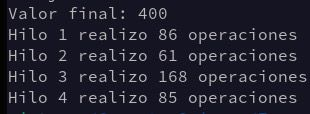
\includegraphics[width = 8 cm]{Images/Practica3_01.jpg}

            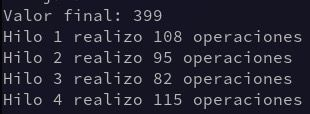
\includegraphics[width = 8 cm]{Images/Practica3_02.jpg}
        \end{center}

        \item De alguna forma obtén el número de veces que los hilos aumentan el contador. ¿Cada uno realiza exactamente 100 tareas o hay algunos que realizan más?

        NO, ya que idealmente deberia de cada hilo hacer 100 tareas pero al los hilos tener diferentes tiempos de hacer sus tareas y su sincronizacion, hay unos que una vez realizan mas o realizan menos, al igual que puede no cumplirse la mutex, porque no tenemos manera de que la seccion critica solo acceda un solo hilo, pongamos el siguiente ejemplo: digamos que tenemos el hilo 1 y 3 donde cada uno toma su candado, lock1 y lock2 exitosamente y estamos en el paso donde nadie ha tomado el lock 3, entonces si ambos llegan a la validacion al lock3 estar libre ambos pasan y entonces ambos entran a la seccion critica, estos casos son raros pero puede pasar y es por ello que tambien llegamos a ver inconsistencias en las tareas.\\


        \item ¿Consideras que la implementación cumple con Justicia? Justifica tu respuesta.

        No, ya que hay hilos que cumplen mas rápido con sus tareas y hay otros aue tardan mas y no se considera eso, ademas que dependiendo del id real de los hilos pueden todos caer en un modulo similar, pero principalmente porque no se toma en cuenta que un hilo lleve esperando un candado.\\
        
    \end{enumerate}

    \hfill

    \item  En base a la implementación de Bakery vista en la clase teoría, implementa Bakery para 4 hilos. \textit{Hint:} Crea los arreglos flag y label de tamaño 4, si consideras necesario utiliza campos volatile

    \begin{enumerate}
        \item Con ayuda de un ExecutorService ejecuta 400 tareas, cada tarea debe aumentar en uno un objeto Contador. Utiliza tu candado para 4 hilos para tener consistencia en tu Contador.

        \item De alguna forma obtén el número de veces que los hilos aumentan el contador. ¿Cada uno realiza exactamente 100 tareas o hay algunos que realizan más?

        \item ¿Consideras que la implementación cumple con Justicia? Justifica tu respuesta.
    \end{enumerate}

    \hfill

    \item Revisa el programa de Bakery que se les compartió como ejemplo, ejecútalo varias veces, revisa el código y contesta:

    \begin{enumerate}
        \item Revisa para que sirve el campo AtomicReference, y qué hacen los métodos compareAndSet() y get().

        Analizando cada elemento por separado:

        \begin{itemize}
            \item AtomicReference nos sirve para realizar operaciones thread-safe (dentro de Java, son las operaciones que se pueden realizar de forma simultánea por parte de varios hilos sin el caer en corrupción de datos o comportamientos no deseados).

            \item El método compareAndSet() nos es de utilidad ya que nos permite de primeras comparar si el contenido de dos elementos (objetos, nodos, etc.) son iguales, y en caso de serlo lo asigna  (en este caso al nuevo nodo) y nos regresa el valor booleano para darnos la idea de si se hizo la operación o no. 

            \item El método get() en este programa lo utilizamos para obtener el nodo deseado según las instrucciones proporcionadas, siguiendo las propiedades de volatile.\\
            
        \end{itemize}

        

        \item Describe como funciona en a lo más 6 líneas de computadora.
        
        Esencialmente, se crea una instancia de Bakery con nodos head y tail y el CounterNaive es compartido por todos los hilos; por cada operación los hilos inicializan un nodo con flag = true y su ID como item, el hilo mediante lock(node) se añade a la ''cola de espera'', este nodo esperará hasta que sea el primero en la cola de espera y que el nodo anterior cambie a flag = false, el hilo incrementa el contador (sección crítica) y termina cuando flag = false, dando paso al siguiente nodo.\\

        \item ¿Si next no es un AtomicReference sigue funcionando? \textit{Hint: Recuerda la Cola concurrente sin candados que implementaste en la Práctica 2}

        Recordando lo visto en la práctica pasada y la función descrita que tiene el campo en si del AtomicReference, podemos decir que next() no funcionaria de la misma manera, lo cual nos llevaría a que tal cual se esta implementando el algoritmo, no sería viable en un entorno concurrente, pudiendo generar fallos en la exclusión mutua, pérdida de nodos, inconsistencias en las listas, etc.\\

        \item ¿Consideras que mantiene la lógica de la implementación vista en clase/tu implementación del ejercicio anterior? Justifica porqué.

        
    \end{enumerate}
\end{enumerate}
